\documentclass{sig-alternate}
\usepackage{epsfig}
\usepackage{algorithm}
\usepackage{algorithmic}

\title{Partitioning a Structured Stream Graph \\ Using Dynamic Programming}
\numberofauthors{1}
\author{
\alignauthor \vspace{-18pt}
William Thies,
Jasper Lin, and
Saman Amarasinghe \\
	\vspace{8pt}
	\{thies, jasperln, saman\}@lcs.mit.edu \\
	\vspace{8pt}
	Laboratory for Computer Science \\
	Massachusetts Institute of Technology}

\begin{document}

  \newtheorem{definition}{Definition}
  \newtheorem{transformation}{Transformation}
  
  \maketitle
  
  \newcommand{\mt}[1]{\mbox{\it #1}}
  \newcommand{\todo}[1]{\framebox{\bf #1}}
  
  \begin{abstract}
    Due to the high data rates involved in audio, video, and signal
processing applications, it is imperative to compress the data to
decrease the amount of storage used.  Unfortunately, this implies that
any program operating on the data needs to be wrapped by a
decompression and re-compression stage.  Re-compression can incur
significant computational overhead, while decompression swamps the
application with the original volume of data.

In this paper, we present a program transformation that greatly
accelerates the processing of compressible data.  Given a program that
operates on uncompressed data, we output an equivalent program that
operates directly on the compressed format.  Our transformation
applies to stream programs, a restricted but useful class of
applications with regular communication and computation patterns.  Our
formulation is based on LZ77, a lossless compression algorithm
utilized by ZIP, and immediately applies to simpler formats such as
Apple Animation, Microsoft RLE, and Targa.

We implemented a simple subset of our techniques in the StreamIt
compiler, which emits executable plugins for two popular video editing
tools: MEncoder and Blender.  For common operations such as color
adjustment and video compositing, computing directly on compressed
data offers a speedup roughly proportional to the overall compression
ratio.  For our benchmark suite of 12 videos in Apple Animation
format, speedups range from 1.1x to 471x, with a median of 15x.

  \end{abstract}

  \section{Introduction}


Stream computing represents an increasingly important class of
applications. In streaming codes, there is an abundance of parallelism that
is easier to extract compared to traditional desktop workloads (e.g.,
pointer-based computing). As a result, the extraction of parallelism
in streaming codes does not require heroic efforts, and thus,
processors can deliver higher performance with significantly lower
power costs. This is especially important since
leading microprocessor companies have realized that modern general
purpose architectures are near their  performance limits for  the
amount of power they consume. Thus, the future will place a greater
emphasis on exploiting the properties of streaming workloads in
conventional von~Neumann architectures.

Streaming is a model of computation that uses sequences of data
and computation kernels to expose concurrency and locality for
efficiency~\cite{wss}. In general purpose processors, improving locality 
translates to an effective management of the memory hierarchy at all
levels, including the register file. In this paper, we present a
methodology for compiling streaming codes to general purpose,
cache-based architectures. We first introduce a simple model for
reasoning effectively about the caching behavior of streaming
workloads. This model serves as a foundation for several {\it cache-aware
optimizations} that are geared toward the concomitant increase of instruction
and data {\it temporal locality}. These
optimization lead to significantly better utilization of the memory
system, and as such, they deliver performance gains ranging from 11
to 99\% for our streaming benchmark suite.

The context for our work is StreamIt, an architecture-independent
language that is engineered for streaming
applications~\cite{streamitcc}. It adopts the 
Cyclo-Static Dataflow~\cite{BELP96} model of computation which is a
generalization of Synchronous Dataflow~\cite{LM87-i} (SDF).  
SDF is a popular  model that  is well suited for
streaming codes. In SDF, computation is represented as a graph
consisting of {\it  actors} connected by communication channels; the
actors consume  and produce a constant number  of items from their
input and output  channels every time they execute. SDF is appealing
because it is amenable to static scheduling and optimization. 

From a general purpose architecture's point of view, actors represent
computation kernels, and the communication between actors represents
data buffers that must be streamed to and from the processor. Thus
the size of an actor and the
order of actor executions are critical properties that
impact the performance of the instruction cache. For example, the
compiler must make sure the actor's code size is not
greater than the instruction cache. Furthermore, we must {\it scale}
the execution of the actor so that it runs several times before we move
on to some other actor in the stream 
graph. This serves to $(i)$ amortize the cost of fetching the actor's
instructions into the cache from memory (an expensive operation), $(ii)$
improve the instruction temporal locality, and $(iii)$ improve overall
performance. However, as our cache model will show, we 
cannot arbitrarily scale the execution frequency of an actor. This
is because actors produce data that must be buffered, and therefore,
we must also consider the amount of data an actor produces and
consumes if we are to adequately manage the data cache. This paper is unique
in that it is the first to present a unified optimization methodology
that simultaneously considers instruction and data locality for
mapping streaming computation to cache-based architectures.

In terms of improving the data cache behavior, the compiler schedules
actor firing such that the producer-consumer locality is
preserved. Furthermore,  the compiler may {\it fuse}
together two or more actors to form a coarser grained kernel.
The fusion allows for better register allocation as we can
destroy the arrays used to buffer data between the actors and replace
the corresponding array references with scalars.  It also allows for
various competing implementations for managing the buffers between the
fused actors.  This paper evaluates several implementation
alternatives (for buffer management) and evaluates their performance.

The methodology for fusing actors leverages a distinguishing StreamIt
characteristic, namely, the hierarchical organization of
the stream graph. Furthermore, the algorithm for fusing actors applies
for the various topologies allowed by StreamIt.
It also considers another distinguishing characteristics of StreamIt,
namely the {\tt peek} operation whereby an actor may inspect data
items in its input buffer without consuming them until some future
execution. While peeking is a powerful language feature, it does pose
some challenges to the compiler and the cache optimizations. Peeking
also impacts the choice for the best buffer management strategy, as our
study will show.

%% the comment about p3 and itanium not being embedded architectures
%% is out of the blue! need a better transition.
Cache-aware fusion alone delivers significant performance gains, although our
evaluation shows that fusion with scaling leads to the best
performance on a general purpose, cache-based architecture. For our
experiments, we use two different processors: a superscalar out-of-order
processor, and an in-order VLIW processor. The former is a Pentium~3
whereas the latter is an Itanium~2. While these architectures are not
particularly suited for an embedded system, they do exhibit some
properties that are worthy of investigation. Furthermore, that we can
demonstrate measurable performance gains on real systems is far more
convincing than using a simulation-based environment. We chose the
Pentium~3 processor because it has very few registers in its
instruction set architecture. The Itanium by contrast has a much 
larger and richer repertoire of registers. The two architectures serve
to validate our cache-aware optimizations, in that we expect an
architecture with more register to benefit more from optimization such
as scalar replacement. On average, fusion leads to a 47\% improvement
on the Pentium~3, and 50\% on the Itanium~2.

The two architectures also differ in terms of their memory system
organization. The Itanium is an in-order VLIW processor and does not
tolerate a memory stall as well as its out-of-order
counterpart. Therefore we expect different gains from the scaling
optimization which amortize the long access latencies for instruction
and data caches. On average, scaling leads to a 21\% improvement on
the Itanium~2, and 17\% on the Pentium~3.

While both scaling and fusion lead to modest performance gains, we
must combine the two to deliver the best possible performance. When we
do so, we can further improve the performance of our benchmarks by
53\% on average for the Pentium~3, and 55\% for the Itanium~2.

\subsection{Summary of Contributions}

This paper makes the following contributions:
\begin{itemize}

\item A cache model for stream computing that provides a quantitative
estimate of the caching performance for any sequence of actor
executions.

\item A cache-aware scheduling heuristic that judiciously increases
the multiplicity of actors, improving instruction and data locality
while not exceeding the data cache.

\item A cache-aware partitioning policy that judiciously fuses
adjacent actors into a single component, enabling local optimizations
while not exceeding the instruction cache.

\item An optimized buffer management policy, termed ``copy-shift with
execution scaling'', which out-performs a traditional rotating buffer
in a detailed micro-benchmark analysis.

\item A fully automatic implementation of the above techniques in the
StreamIt compiler.

\item An experimental evaluation across 11 streaming benchmarks,
demonstrating performance improvements of up to 99\%.
\end{itemize}

\subsection{Paper Roadmap}

The remainder of the paper is organized as follows. Section~\ref{sec:streamit}
describes StreamIt and introduces our motivating example.
Section~\ref{sec:cache-model} introduces our cache model for 
reasoning about the performance of a streaming
computation. Section~\ref{sec:cache-opt} describes our cache-aware
optimizations, and Section~\ref{sec:buffer} describes the 
optimization enabled by fusion. Section~\ref{sec:evaluation} describes
our evaluation methodology and present our experimental
analysis. Sections~\ref{sec:related-work}~and~\ref{sec:conclusion}
discuss related work and concludes the paper.

  \section{StreamIt}
\label{sec:streamit}

StreamIt  is   an  architecture-independent  language that was
designed for  streaming applications. In StreamIt, programs are
represented as graphs where  nodes represent  computation and edges
represent FIFO-ordered communication of data over tapes.

The  basic programmable  unit (i.e., an actor) in  StreamIt is a {\it
filter}.   Each filter contains  a work  function that executes
atomically,  popping (i.e., reading)  a fixed number  of items  from
the  filter's input  tape and pushing (i.e., writing) a fixed number
of items to the filter's output tape.  A filter  may also {\tt peek} at
a given index  on its input tape without  consuming  the  item;  this
makes  it  simple  to  represent computation over a
sliding-window.   The {\tt push}, {\tt pop}, and {\tt peek} rates are
declared as part  of  the work  function,  thereby enabling  the
compiler    to construct a static schedule of filter executions. The
following is an example implementation of a FIR   (Finite Impulse
Response)  filter: 
%\begin{scriptsize}
{\small
\begin{verbatim}
float->float filter FIR (int N, float[] weights) 
{
  work push 1 pop 1 peek N {
    float sum = 0;
    for (int i = 0; i < N; i++) {
      sum += peek(i) * weights[i];
    }
    pop();
    push(sum);
  }
}
\end{verbatim}}
%\end{scriptsize}

The work function is invoked (fired) whenever there is sufficient data
on the input tape. In this case, the filter requires at least
\texttt{N} elements before it can execute. The value of \texttt{N} is
known at compile time when the filter is composed to form a stream
graph. A filter is akin to a class in object oriented programming
with the work function serving as the main method. The parameters
to a filter (e.g., \texttt{N} and \texttt{weights}) are equivalent to
parameters passed to a class constructor. In StreamIt, the
application developer focuses on the hierarchical assembly of the
stream graph and its communication topology, rather than on the 
explicit management of the data buffers between filters.

\begin{figure}[t]
\begin{center}
\vspace{-24pt}
 \framebox{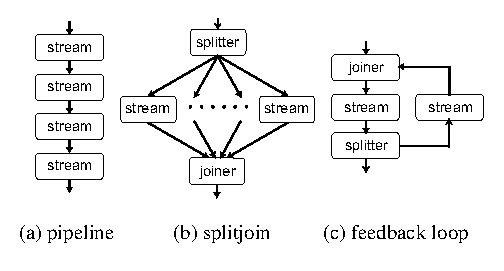
\includegraphics[scale=1, angle=0]{./constructs-eg.eps}}
 \vspace{-6pt}
 \caption{StreamIt containers.}
 \label{fig:containers}
\end{center}
\end{figure}

\begin{figure}[t]
\begin{center}
\vspace{-12pt}
 \framebox{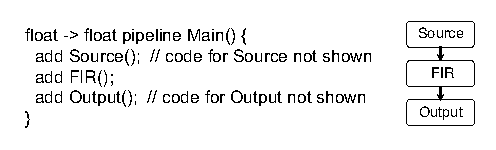
\includegraphics[scale=1, angle=0]{./pipeline-eg.eps}}
 \vspace{-6pt}
 \caption{Example pipeline with FIR filter.}
 \label{fig:pipeline}
\vspace{-18pt}
\end{center}
\end{figure}

StreamIt provides three hierarchical structures for composing filters
into larger stream graphs (see Figure~\ref{fig:containers}). The 
{\it pipeline} construct composes streams in sequence, with the output
of one connected to the input of the next.   An example of a pipeline
appears in Figure~\ref{fig:pipeline}.

The {\it splitjoin} construct distributes data to a set of parallel
streams, which are then joined together in a round robin fashion.  In
a splitjoin, the {\it splitter} performs the data scattering, and the
{\it joiner} performs the gathering. A splitter is a specialized
filter with a single input and  multiple output channels. On 
every execution step, it can distribute its output to any one of
its children in either a {\it duplicate} or a {\it roundrobin}
manner. For the former, incoming data is replicated to every
sibling connected to the splitter. For the latter, data is scattered
in a round-robin manner, with each item sent to exactly one child
stream, in order.  The splitter type and the weights for distributing data to
child streams are declared as part of the syntax (e.g., \texttt{split
duplicate} or \texttt{split roundrobin($w_0$, $w_1$, ... $w_n$)}). The
splitter counterpart, the joiner, is a specialized filter with  
multiple input channels but only one output channel. The joiner
gathers data from its predecessors in a round-robin manner (declared
as part of the syntax). 

StreamIt also provides a {\it feedback loop} construct for introducing
cycles in the graph.

\section{Execution Model}
\label{sec:execmodel}

A StreamIt program is represented by a hierarchical graph,
where the leaf nodes are filters, splitters, and joiners, and
the composite nodes are pipelines, splitjoins, and
feedback-loops. Edges in the graph represent data channels, which 
operate as FIFO queues.
In order for an actor  (i.e., a filter,
splitter, or joiner) to execute, it must have enough data items on its input
tape. In StreamIt, actors have  two epochs
of execution: one for initialization, and one for the steady
state. The initialization primes the input tapes to allow filters with
peeking to execute the very first instance of their work functions;
initialization in this setting is similar to the prologue stage in
software pipelining. The steady state schedule has the property that
the amount of data buffered between any two actors does not change
before and after the actor executions.

\begin{figure}[t]
\begin{center}
\vspace{-24pt}
 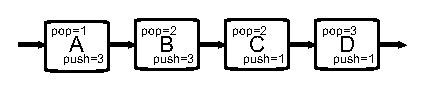
\includegraphics[scale=1, angle=0]{./pipe-with-rates.eps}
\vspace{-6pt}
 \caption{Example pipeline.}
 \label{fig:pipe-with-rates}
\end{center}
\end{figure}

As an example, a steady state schedule for the sample pipeline in
Figure~\ref{fig:pipe-with-rates} requires filter \texttt{A} to fire
four times, \texttt{B} six times, \texttt{C} nine times, and
\texttt{D} three times. 
% Because in StreamIt the filters are
% independent (i.e., they do not share state), they can execute
% concurently. In a uniprocessor setting (which is what we use for our
% evaluation), we can only run one filter at time. Therefore, 
The data generated by one actor is buffered (cached) until it is
consumed.

The StreamIt compiler derives the initialization and steady state
schedules~\cite{karczma-lctes03} and outputs a C program that includes
the initialization and work functions, as well as a driver to execute
each of the two schedules. For example, referring to
Figure~\ref{fig:pipe-with-rates}, the compiler generates the following
sample code for running the steady state schedule:
%\begin{scriptsize}
\begin{verbatim}
run_steady_state() {
  for (i = 0; i < 4; i++) A_work();
  for (i = 0; i < 6; i++) B_work();
  for (i = 0; i < 9; i++) C_work();
  for (i = 0; i < 3; i++) D_work();
}
\end{verbatim}
%\end{scriptsize}
To execute the program, the steady state kernel is wrapped with
another loop that invokes the kernel a designated number of
times. Preceding the state steady, a similar initialization schedule
is run to prime the data buffers, and following the steady state, an
epilogue is run to drain the buffers as necessary.

\begin{figure}[t]
\begin{center}
\vspace{-12pt}
 \psfig{figure=ssi.eps,width=3in}
 \vspace{-6pt}
 \caption{Instruction size (in bytes along the y-axis) per filter
 (x-axis) occurring in a steady state execution of FFT.}
 \label{fig:ssi-single}
\vspace{-18pt}
\end{center}
\end{figure}

From a caching point of view, it is intuitively clear that once a
filter's instruction working set is fetched into the cache, we must
execute that filter as many times as possible to improve instruction
locality and amortize the cost of the accesses to lower levels of the
memory hierarchy. This of course assumes that the total code size for
the filters in the steady state exceeds the capacity of the
instruction cache (which is commonly the case;). In
Figure~\ref{fig:ssi-single} we show a representative breakdown of the
code size per filter in a steady state execution of a StreamIt
implementation of FFT. In all, the total code size for a steady state
ranges from 16~Kb to over 60~Kb for our benchmarks. These results
provide evidence that while individual filters may have a
small instruction footprint, the total footprint of the filters in a
steady state exceeds a typical instruction cache size.
From these observations, it is evident that we must {\it scale} the
execution of filters in the steady state in order to improve temporal
locality. In other words, rather than running a filter $S$ times per
steady state, we increase the loop bound so that it runs $\texttt{M}
\times S$ times (e.g., the loop bound for \verb+A_work+ is
changed to $\texttt{M} \times 4$ in the example shown earlier). 
We term \texttt{M} the {\it multiplicity factor}.

The obvious question is: to what extent can we scale the execution of
filters in the steady state? The answer is non-trivial because
scaling, while beneficial to the instruction cache behavior, may
overburden the data cache as the buffers between actors may grow to
prohibitively large sizes that degrade the data cache
behavior. Specifically, if a buffer overflows the cache, then
produce-consumer locality is lost. 

Also complicating matters is the amount of state a filter must retain
from one execution of its work function to the next. In the FIR
example shown earlier, the filter state is proportional to the size of
the coefficient array (i.e., \texttt{weights}). The filter state
further constrains the schedule scaling.

  \section{Graph Transformations}
\label{sec:transforms}

In this section we present a set of flexible transformations that can
be used to adjust the hierarchy and communication patterns of a
structured stream graph.  These transformations serve two purposes.
Firstly, they provide a means of deriving a canonical form: a program
representation that is insensitive to changes in the source code and
is easily analyzed by the compiler (for example, the hierarchical
ragged arrays of the partitioner).  Secondly, they serve as the
implementation mechanism by which the compiler arrives at an efficient
executable once it has analyzed the canonical form (for example, the
partitioner's traceback function).

Thus, we consider the transformations in pairs, each of which
represents a step in the opposite direction with respect to the
partitioner's representation.  After describing the transformations,
we describe the sequence in which they are employed when interfacing
to and from the partitioner.

\subsection{Vertical Cut Transformations}

The vertical cut transforms effect the distribution of parallel
streams across a hierarchy of splitjoin constructs (see
Figures~\ref{code:vert} and~\ref{ex:vert}).  The {\tt lowerChildren}
transform can factor any adjacent subset of a splitjoin's children
into a new splitjoin, which becomes a child of the original.  This is
a simple matter of re-arranging the weights in the splitters and
joiners.  It qualifies as a ``vertical cut'' transform because two
adjacent applications can divide a splitjoin with a vertical line.

The {\tt raiseChildren} transform will reverse the effect of any {\tt
lowerChildren} transform.  However, independent applications of this
transform are comparably rare: as detailed in the pseudocode, a child
can only be raised if its splitter type matches that of its parent,
and if the sums of its split and join weights match the corresponding
slots in the parent.

\subsection{Horizontal Cut Transformations}

The horizontal cut transforms are capable of transforming between a
splitjoin and a pipeline of splitjoins (see Figures~\ref{code:horiz}
and~\ref{ex:horiz}).  The {\tt addMatchingSyncPoints} transformation
inputs a rectangular splitjoin--one with pipeline children that have
equal lengths--and factors them into a sequence of splitjoins with
children that have unit length.  For the purpose of program analysis,
any splitjoin can be made rectangular by extending its shorter streams
with {\tt Identity} filters (a pre-defined node in StreamIt.)  Like an
hourglass, this transformation has the effect of squeezing a splitjoin
together at points of synchronization.

The {\tt removeMatchingSyncPoints} transformations directly implements
the inverse of {\tt addMatchingSyncPoints} via a simple re-arrangment
of weights.  Though very simple, this transformation can apply in
practice on interface boundaries where compound data streams are being
interleaved at a static rate.

A more aggressive transformation for synchronization removal is {\tt
removeStructuredSyncPoints} (see Figures~\ref{code:sync}
and~\ref{ex:sync}).  This algorithm removes not only synchronization
points with exactly matching weights, but it also expands any
join/split pair where the set of incoming and outgoing streams can be
partitioned such that no data item is passed between members of
different partitions during a steady-state execution.  The only
disadvantage of this transformation over {\tt
removeMatchingSyncPoints} is that it has the potential to introduce
non-adjacent joiners, which in the StreamIt compiler requiers
additional processor resources.  However, like all transformations
described in this paper, the output of {\tt
removeStructuredSyncPoints} is still a structured graph (as the name
would suggest).

We have also implemented horizontal cut transforms for pipelines,
which consist simply of adding or removing a wrapper pipeline around a
sub-segment of the stream.  This is very straightforward (requiring no
change of weights or rates) so we ommit the details here.

\subsection{Fusion and Fission Transformations}

Filter fusion describes a transform where several adjacent filters are
combined into one, while filter fission refers to the parallelization
of a filter via conversion to a splitjoin or pipeline.  These
transformations are at the heart of the load balancing partitioner
described in this paper.  A detailed description of fusion, fission,
and other intra-node transformations are described
in~\cite{streamit-asplos}; we restrict our attention to graph-level
transformations in this paper.

\subsection{Transforming to Partitioner's Representation}

To build the hierarchical arrays required by the partitioner, the
following transformations are applied, starting from the leaf nodes
and propagating upwards through the stream:
\begin{itemize}

\item {\tt raiseChildren} and {\tt removeStructuredSyncPoints}
wherever possible.

\item {\tt removeMatchingSyncPoints} wherever possible.

\item Convert all non-rectangular splitjoins to rectangular ones by
extending their shorter child pipelines with Identity filters.

\item {\tt addMatchingSyncPoints} on all splitjoins.
\end{itemize}

The last step above will have the effect of replacing every splitjoin
with a pipeline of unit-length splitjoin constructs.  This pipeline is
exactly the representation that is sent to the partitioner; the width
of row {\tt y} is the width of the splitjoin at that location.  

\subsection{Transforming from Partitioner's Representation}

The traceback function is what calculates the sequence of
transformations needed to trasnform from the partitioner's
representation to the load-balanced set of partitions for program
execution.  In Figure~\ref{code:trace}, the points corresponding to a
vertical and horizontal cut are where traceback recurses after finding
the optimal {\tt xPivot} (for vertical cut) or {\tt yPivot} for
horizontal cut.  In our implementation, these cuts are recorded during
traceback, and then replayed on the stream graph at a later time.  The
only extra step to take is that synchronization must be removed before
any vertical cut is applied.

An example of the conversion to and from the partitioner's
representation appears in Figure~\ref{fig:trans}.


  \section{Partitioning Algorithm}

In this section we describe our partitioning algorithm, which operates
on an abstract representation of the stream graph and is well-suited
for many interesting problems.

\subsection{Problem Definition}

In this paper we focus on a static load-balancing problem, which we
define as follows.  We are given the following:
\begin{itemize}

\item A StreamIt stream graph $\mt{str}$ in which each filter $filter$
has a certain amount of steady-state $\mt{work}$ and can be run in
data parallel (to an arbitrary degree) if $\mt{isFissable(f)}$ is
true.

\item An integer $N$ denoting the number of available partitions.

\end{itemize}

The goal is to produce a mapping $\mt{map}$ from nodes to partitions
that minimizes the cost of the bottleneck node {\it while maintaining
a structured stream graph}.  Formally, this could be posed as:

%% \begin{center}
%% \framebox{
%% Minimize $MAX_{i}  (\sum_{d \in \{ d~|~map(d)=i\}} d.work)$
%% Subject to:
%% \begin{enumerate}

%% \item Every node is assigned to a legal partition:
%%   \[
%%   \forall d \in s:~~ 0 < \mt{map}(d) < n
%%   \]

%% \item There exists a structured stream graph with the same.
%% \end{enumerate}}
%% \end{center}


\subsection{Converting to the Canonical Form}


\subsection{Implementing the Transformations}




operates on an abstract representation of the stream graph to

exploits
the hierarchical structure of the stream graph


canonical representation
- maintains single-input, single-output

advantages of this algorithm:
 - canonical form
  - cuts along important places, in right directions
  - detecting symmetry and hierarchy to save time
    - work estimation
    - alisasing of child configurations
    - evaluating child configurations themselves

- does fissoin and fusion
- sticks with space multiplexing

- show how we can provide rectangular abstraction on single-input, single-output streams

  - partitioner takes advantage of this in two ways: 
    1) by detecting symmetry and only calculating things once
    2) by drawing cuts along likely paths
    3) by automatically calculating some properties that are the best,
       e.g. if you have the same filter duplicated in a splitjoin

- two thrusts: that structure actually SUPPORTS powerful ways of
program reasoning, and that we are flexible enough to manipulate
structured programs into a number of isomorphic forms.  can consider
structures on an abstract level, and then implement them in any number
of ways.

- very fast?  no

  \section{Evaluation}
\label{sec:eval}

In this section we evaluate the framework presented in this paper.  We
have implemented the techniques in the context of the StreamIt
compiler infrastructure~\cite{gordon-asplos06}.  The fission and
sharing reduction techniques are guided by the parallelization
management algorithms covered in~\cite{gordon-asplos06}.  These
algorithms offer a holistic approach to exploiting coarse-grained
task, data, and pipeline parallelism.   Once, the parallelization management
algorithm decides how to exploit data-parallelism, i.e., which
filters should be data parallelized and by what degree, our fission
algorithm of Section~\ref{sec:data-par} is utilized to perform the
data-parallelization. 

We compare our techniques to previously published techniques for
fission of sliding window filters that perform duplication of all
input items and decimation of unneeded items (DupDec).  We employ
three benchmarks for the evaluation.  The ChannelVocoder benchmark is
the analyzer portion of a source-filter model speech coder.  The
Filterbank benchmark implements a multi-rate signal decomposition
processing block common in communications and image processing.  The
FMRadio benchmark implements an FM radio with multi-band equalizer.
The following table provides more details on the benchmarks:


{\centering
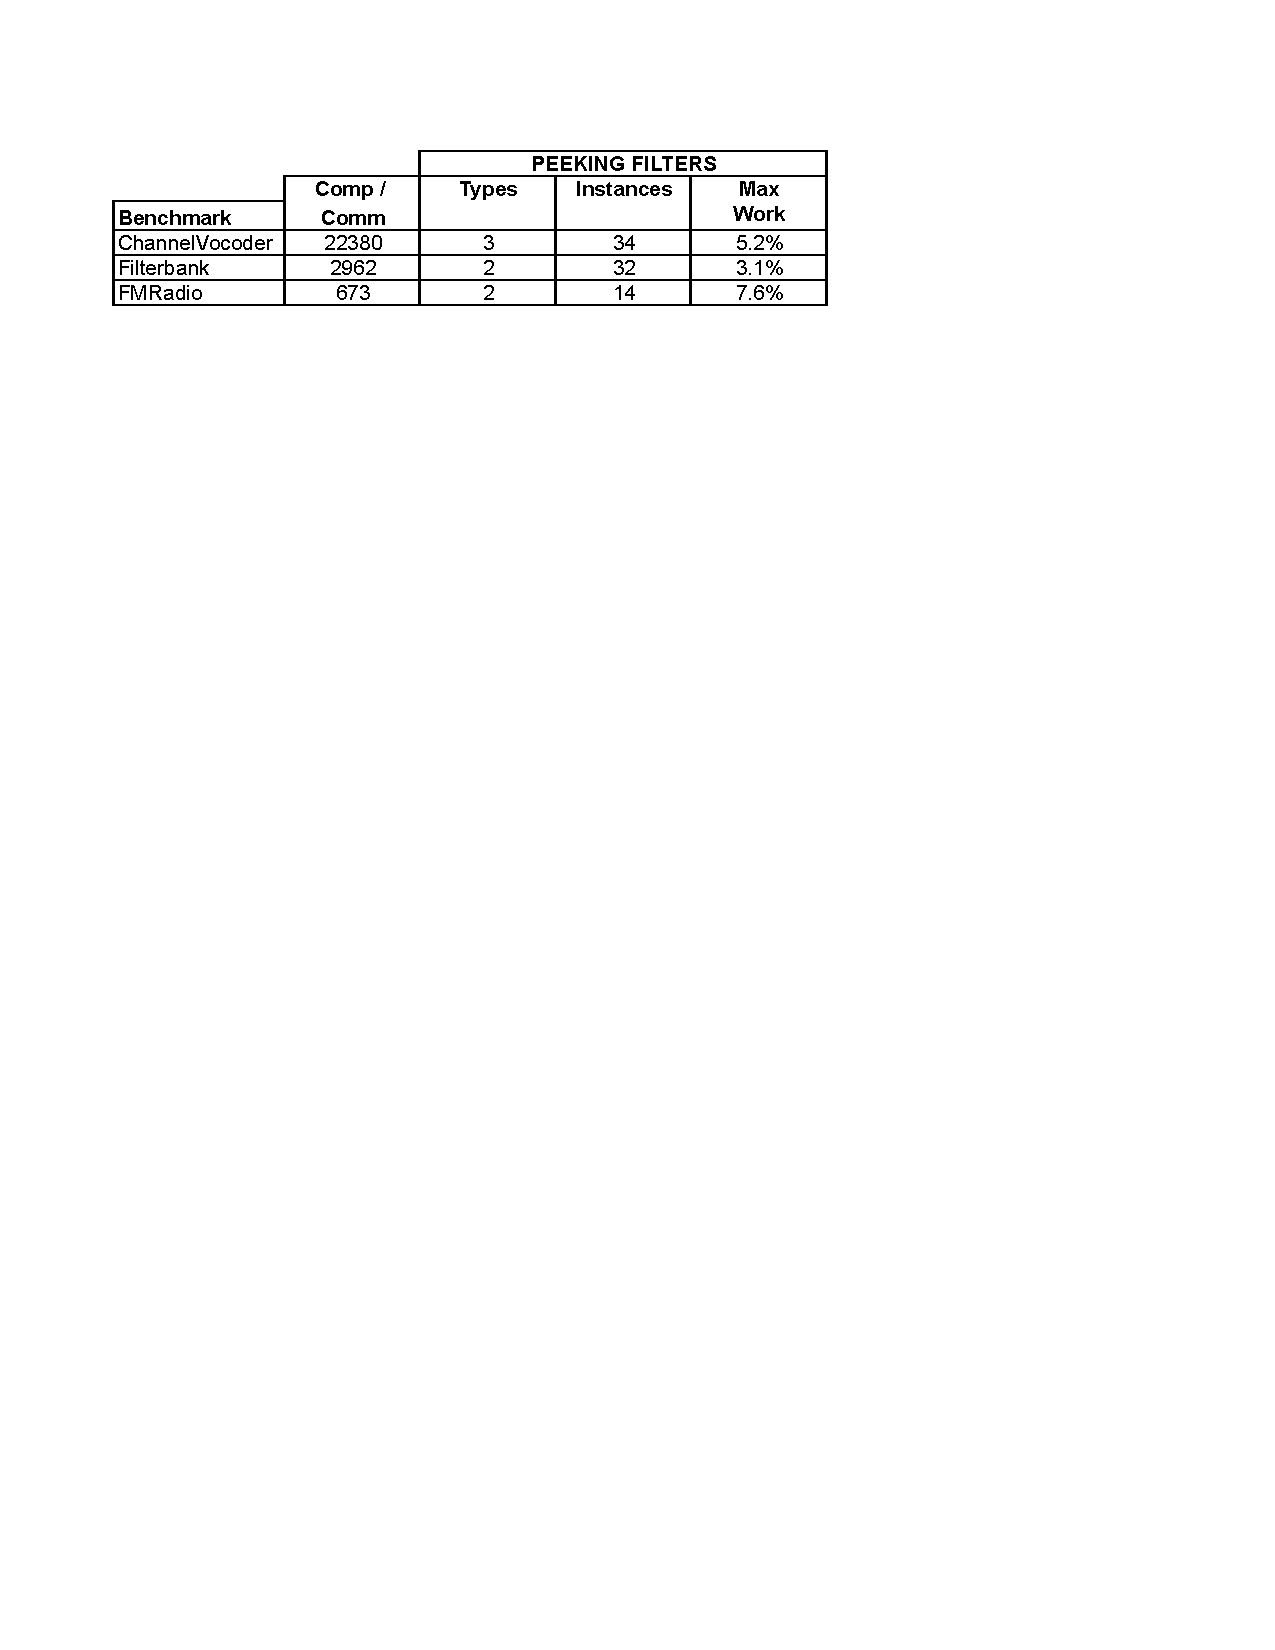
\includegraphics[width=3.3in]{figures/bench-char.pdf}}

\noindent ``Comp/Comm'' provides a static estimation of the
amount of computation to communication ratio by statically estimating the total
work of all the filters and dividing by the number items communicated
for the programmer-conceived graph's steady-state.  The remaining
statistics give the number of peeking filters types, number of peeking
filters instantiated at runtime, and a static estimation of the maximum
work in the single most loaded peeking filter.

We target 2 multicore architecture with different communication
mechanisms.  The Tilera Corporation's TILE64 Processor is a 64 core
system on a chip~\cite{tilera}.  Each core is an identical three-wide
VLIW. The code generated by the StreamIt
compiler for the TILE64 processor follows the remote store programming
(RSP) model~\cite{rsp10} in which each process has a private address
space, but each process can award remote processes write access to
their local memory. When a producer process has write access to a
consumer process's memory, the producer communicates directly with the
consumer via store instructions whose destination is an address in the
consumer's shared memory.  Communication is initiated by the producer,
and is fine-grained.  The consumer reads directly from it's local
memory (L2) when accessing input.

Our symmetric multiprocessor target is a 16-core architecture that is
comprised of four Intel Xeon E7350 multicore processors.  Each processor
is a 64-bit, quad-core with two dual-core dies.  Each die contains a 4
MB L2 cache shared across the two cores.  The front-side bus is clocked
at 1066 MHz.  We utilize the cache coherency mechanism of the
architecture for communication between cores. 

Through empirical experimentation on FMRadio, Filterbank, and
ChannelVocoder, we have settled on $T_{\mt{sharing}} =.10$ and
$T_{\mt{apply}} = 0.05$. These constants are the sweet stop for the two
architectures employed in the experimentation, being a good compromise
between buffer size and inter-core communication.

% \begin{figure*}[t]
% \centering
% \subfigure[]{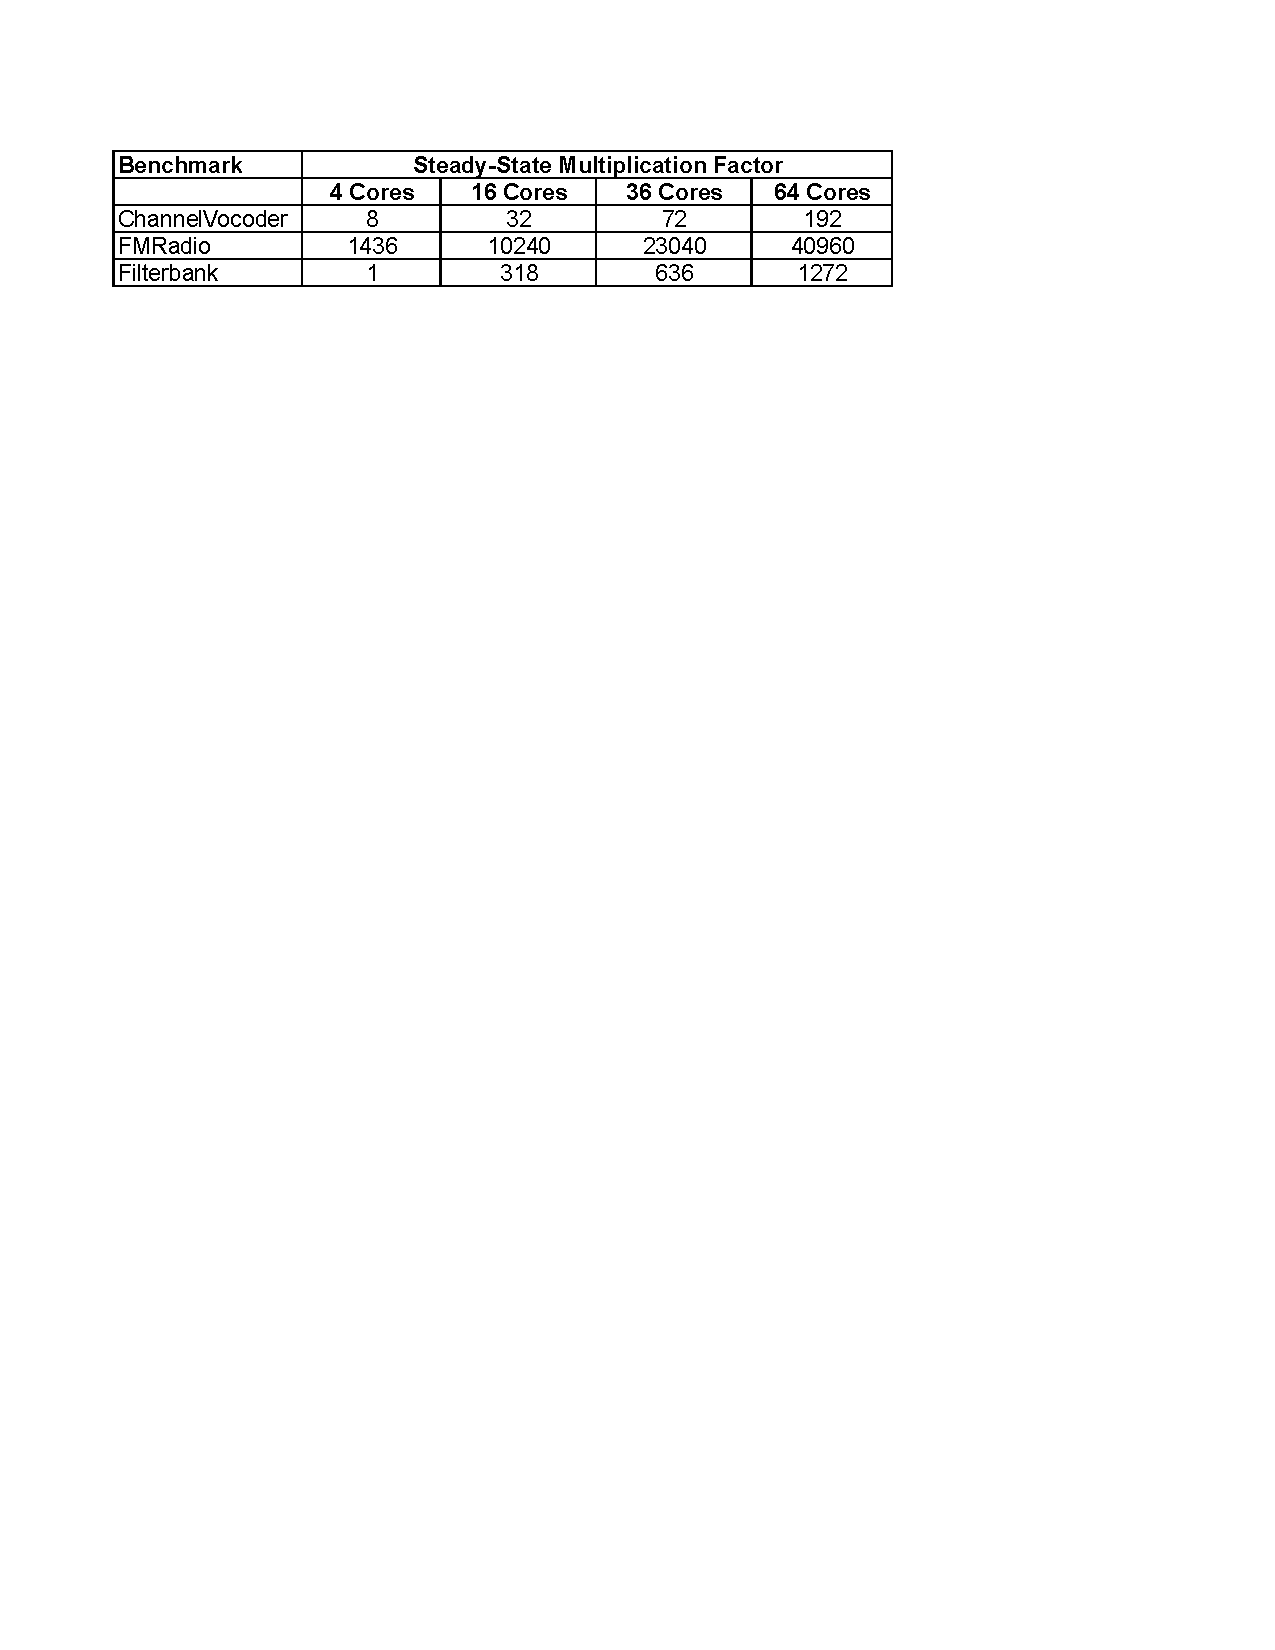
\includegraphics[width=3.7in]{figures/mult-table.pdf}} \\
% \subfigure[]{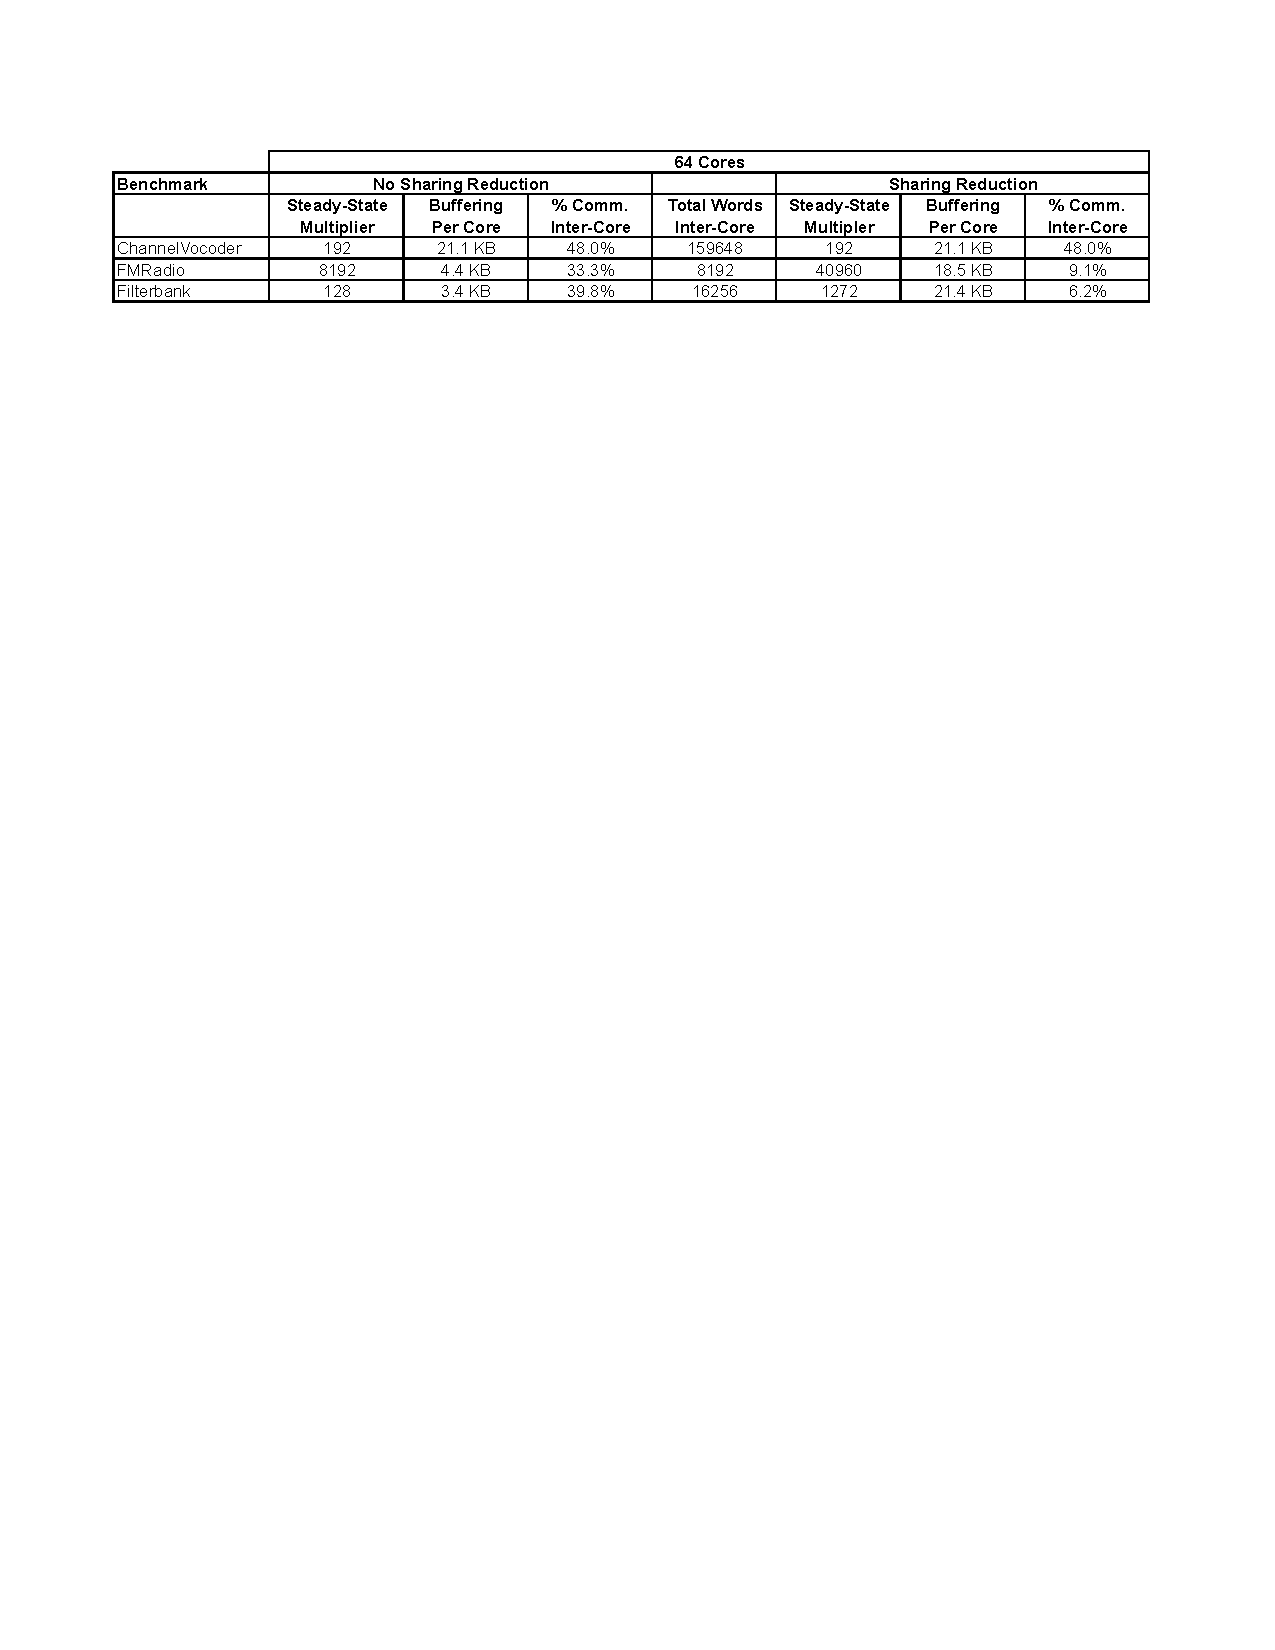
\includegraphics[width=6in]{figures/64-core-table.pdf}}
% \caption[Communication, multiplier and buffering statistics for
% benchmarks.]{
% Communication, multiplier and buffering characteristics for
% benchmarks: (a) gives the steady-state multipliers calculated for
% sharing reduction, (b) compares the steady-state with and without
% sharing reduction. 
% \label{fig:fission-table}}
% \end{figure*}

\begin{figure*}[t]
\centering
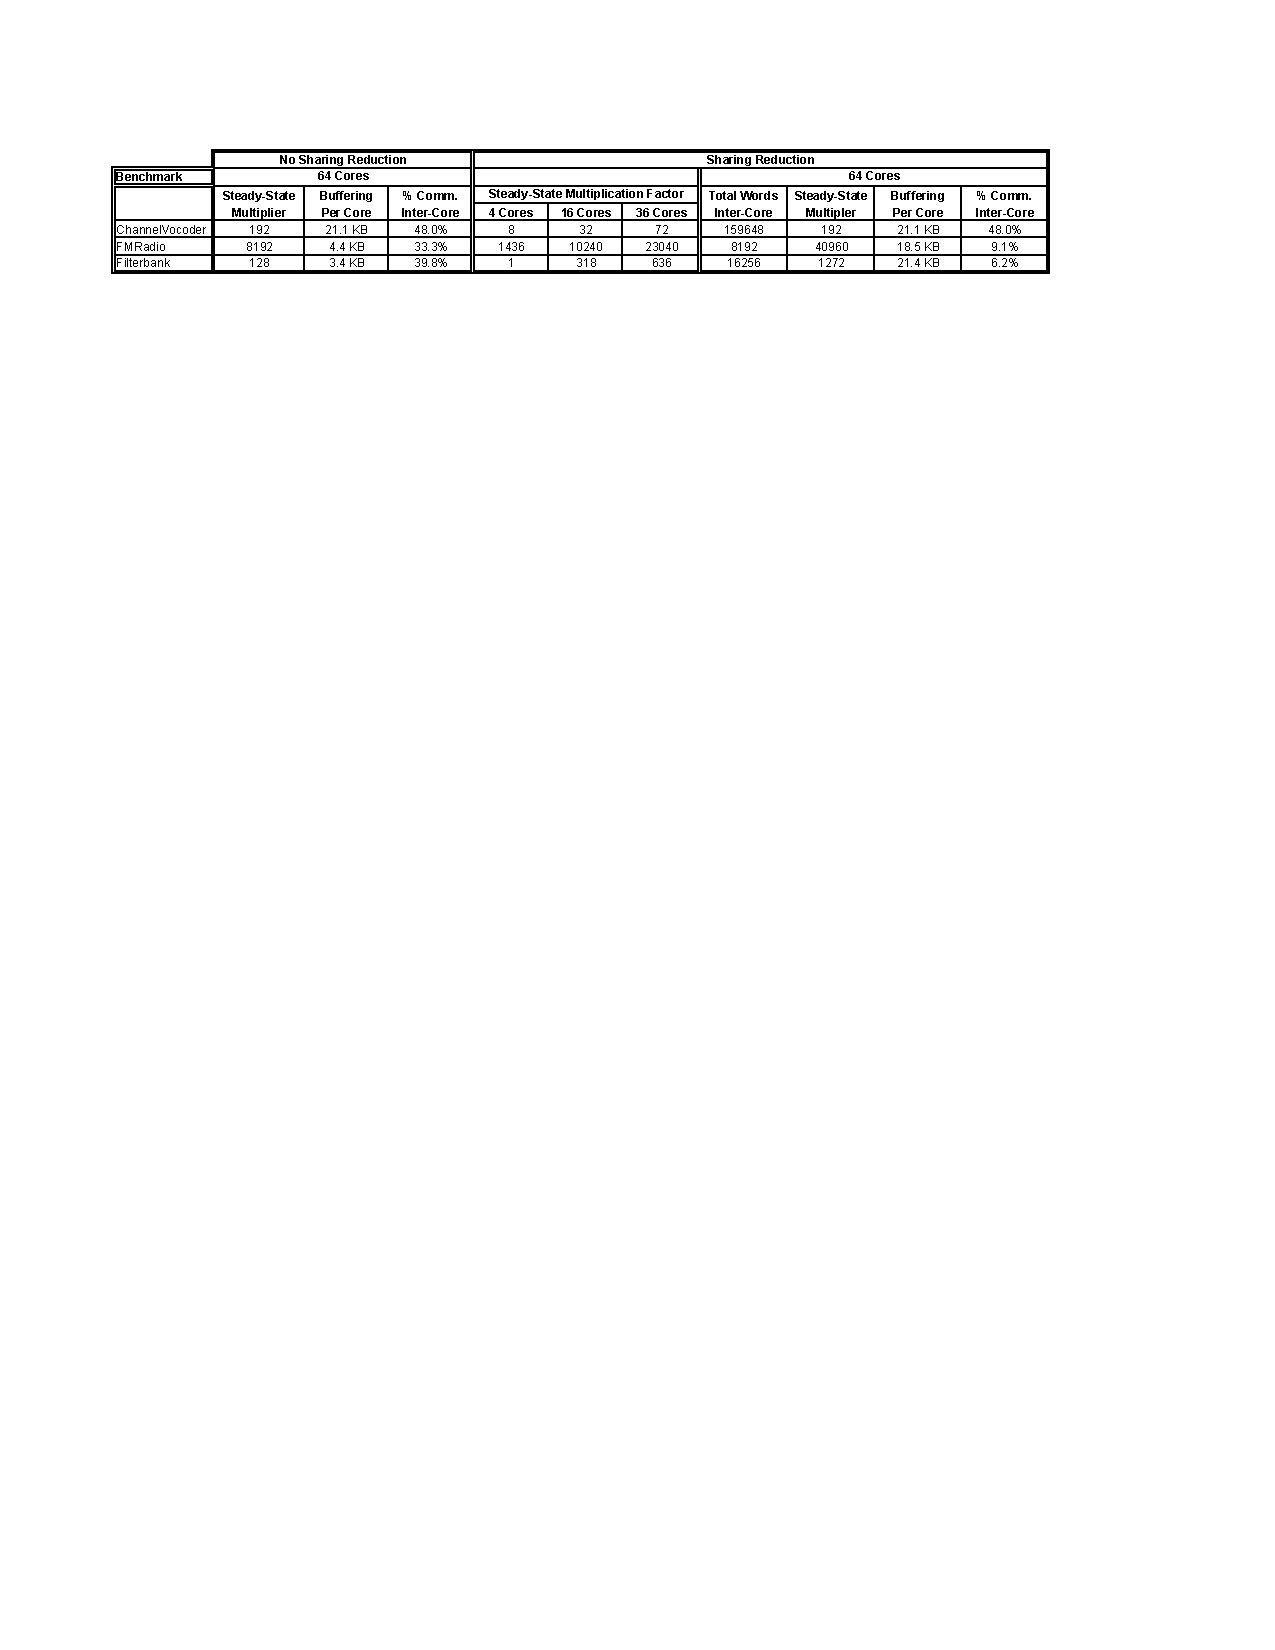
\includegraphics[width=6.1in]{figures/big-table.pdf}
\caption{\label{fig:big-table}  Steady-state multiplicity, buffering,
  and communication for fission with and without sharing reduction.}
\end{figure*}

% \begin{figure}[t]
% \centering
% 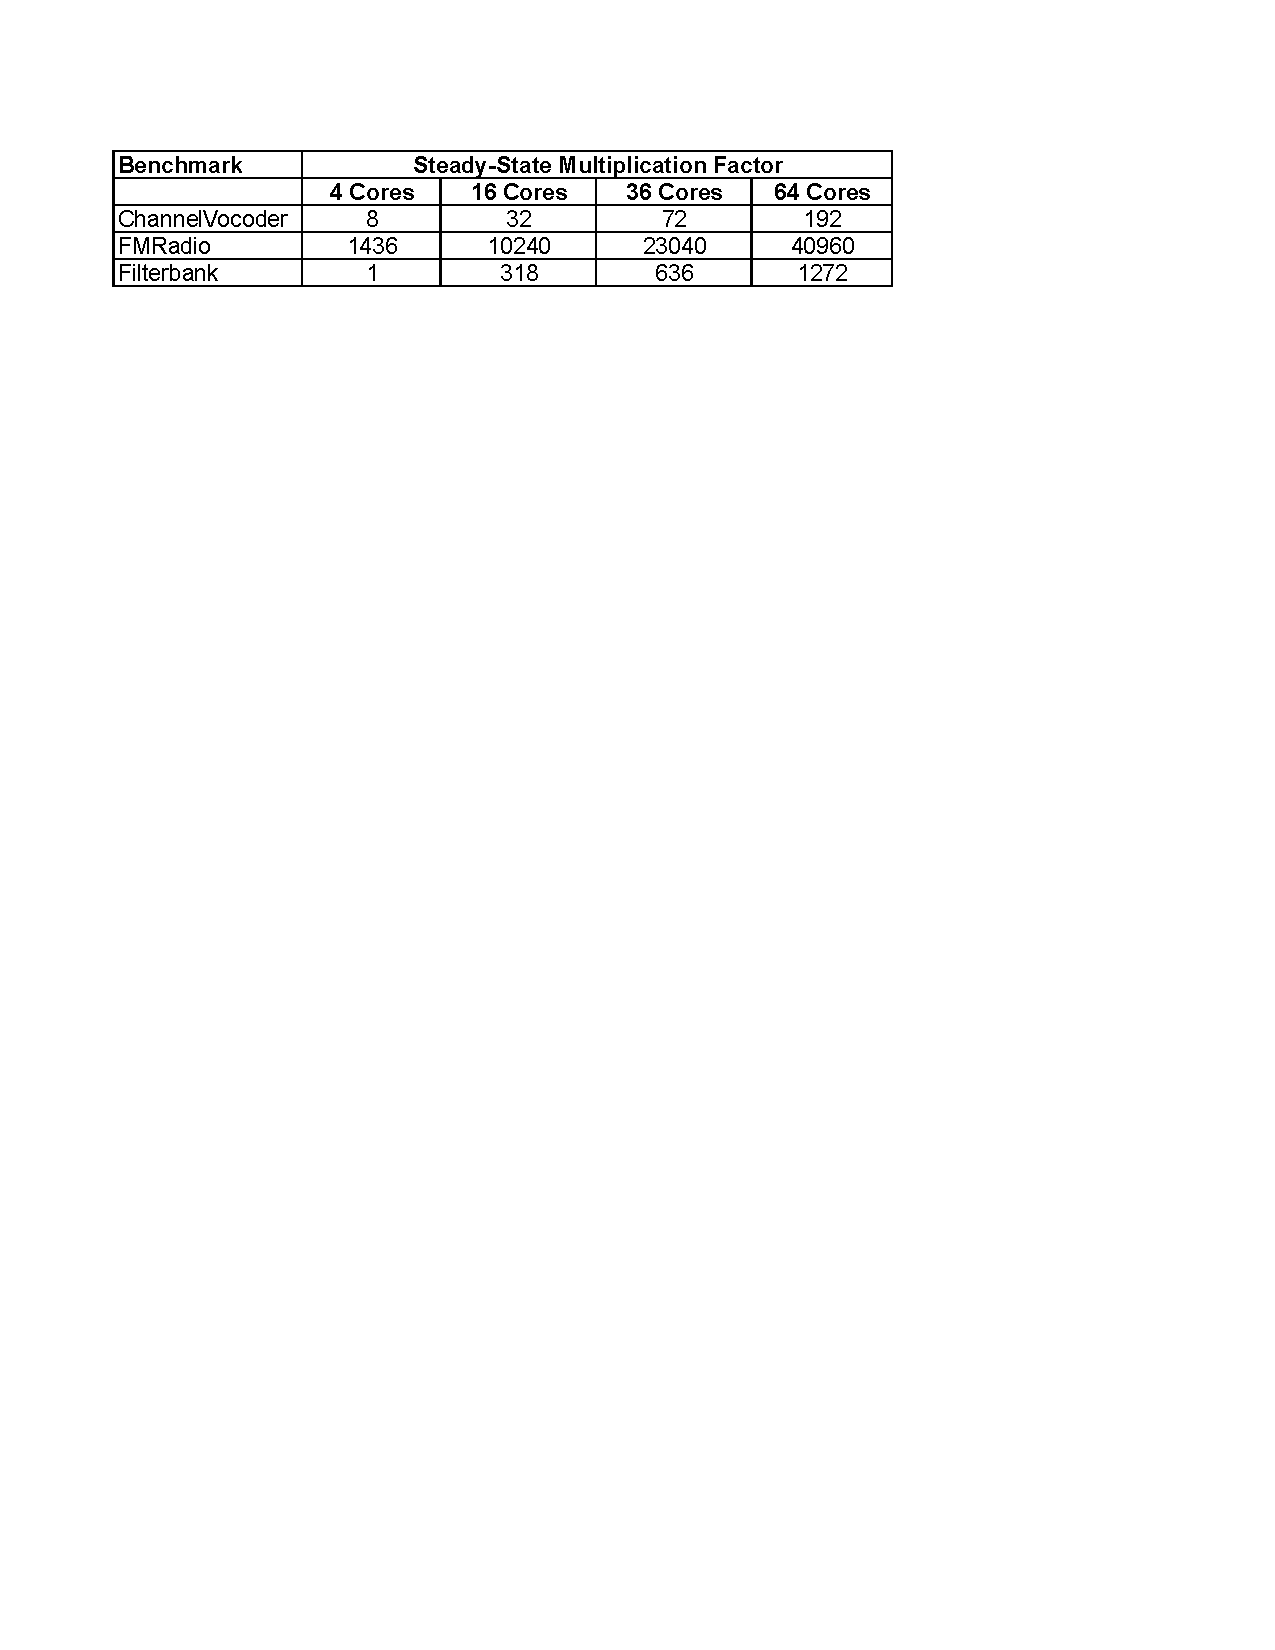
\includegraphics[width=3.3in]{figures/mult-table.pdf}
% \caption{\label{fig:mult-table}  The steady-state multipliers calculated for
% sharing reduction.}
% \end{figure}

% \begin{figure*}[t]
% \centering
% 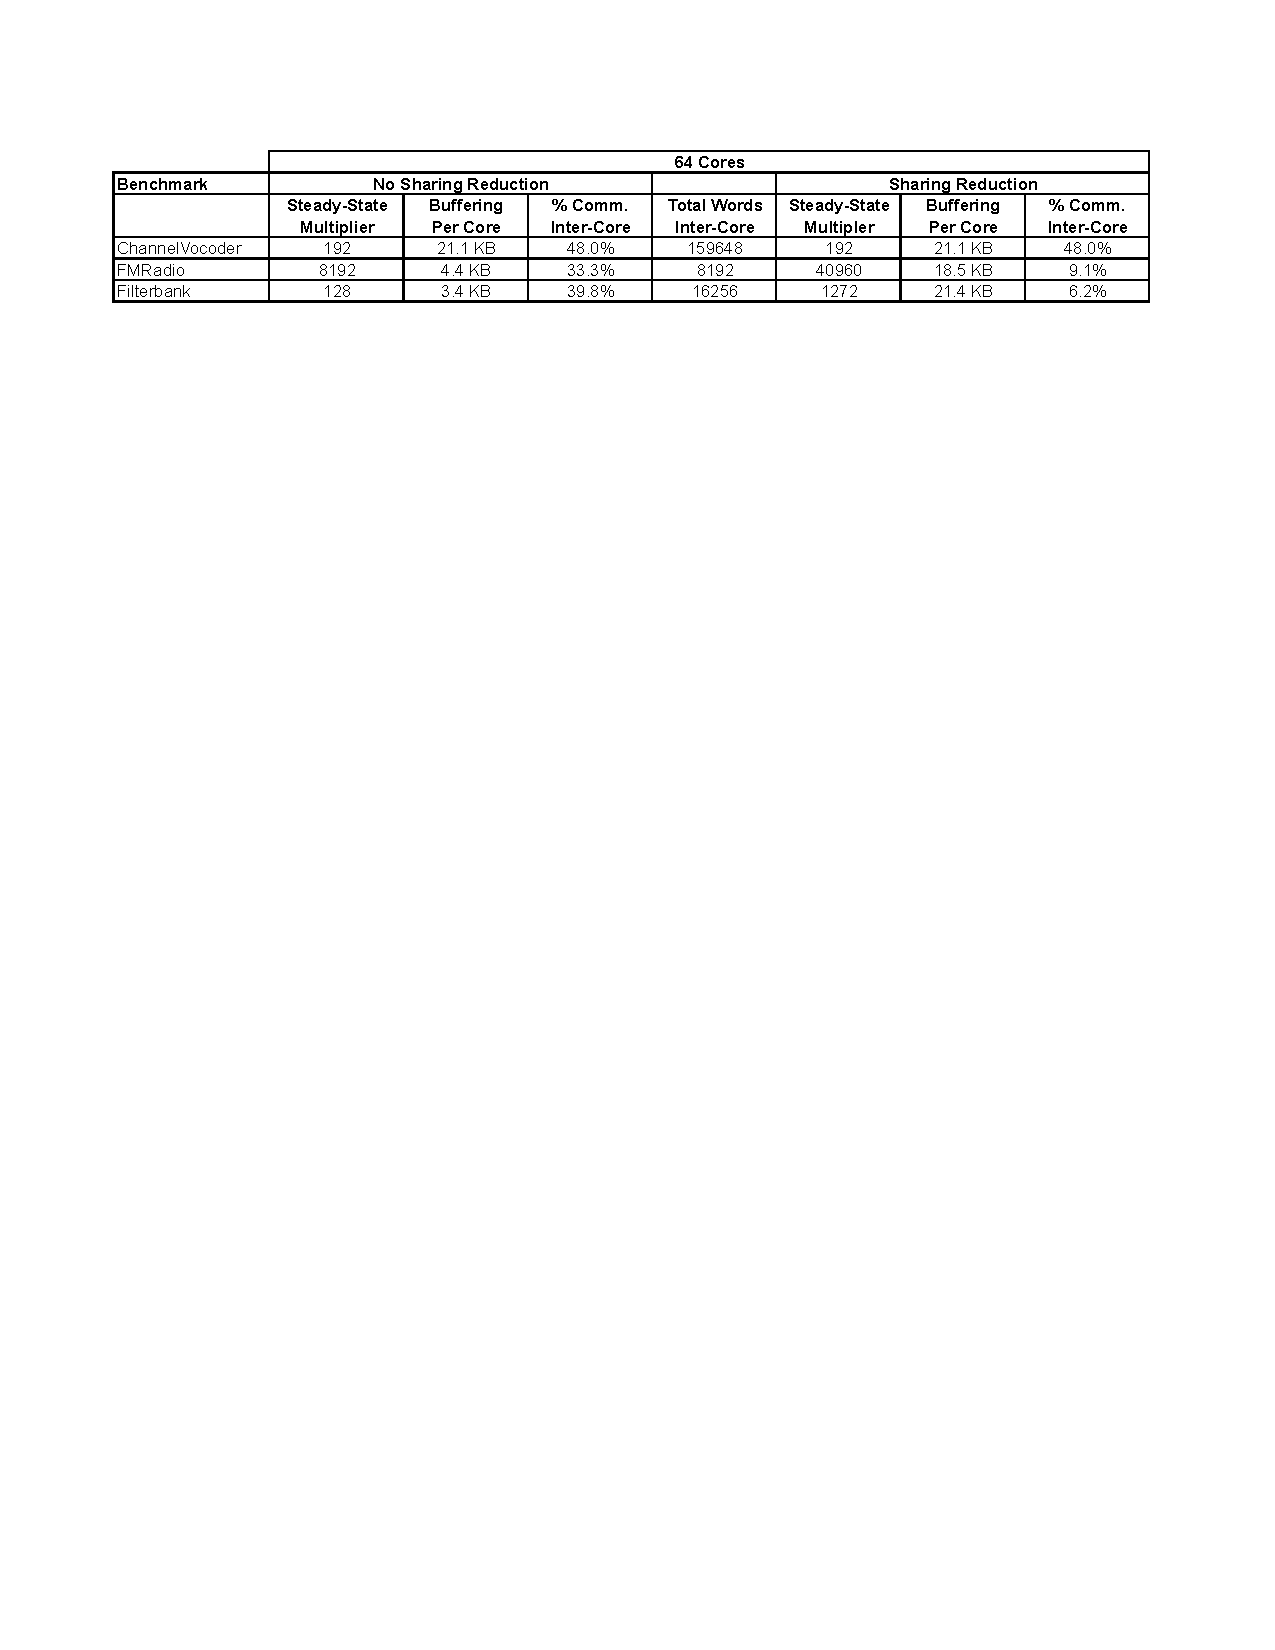
\includegraphics[width=6in]{figures/64-core-table.pdf}
% \caption{ Multiplier, buffering and communication for the steady-state with and without
% sharing reduction. 
% \label{fig:fission-table}}
% \end{figure*}

Figure~\ref{fig:big-table} compares the steady-state with and
without sharing reduction for a 64-core mapping, as well as gives the
constant $c$ calculated by sharing reduction for 4, 16, and 36.  The
factor is larger for FMRadio because one filter has $C(f) \gg o(S,
f)$.  The multiplication factor affects both latency and buffer sizes
adversely.  The application designer will have to decide if the
latency of these techniques can be borne given the application
criteria.  The total buffering requirement is increased when the
steady-state is increased.  However, since we are then fissing, the
buffer is divided amongst the fission products, and the {\it per-core}
buffering requirement is unaffected by the increase.  For example,
FMRadio, has a per-core 18 KB buffering requirement across all
configurations (4, 16, 36, and 64 cores).  This requirement fits in
the per-core L2 size of 64 KB for the Tile64.

 For ChannelVocoder,
sharing reduction has no effect because most of the peeking filters do
not satisfy $T_{\mt{apply}} = 0.05$ because of differing fission
factors between producers and consumers.  For the peeking filters that do,
the steady-state multiplier required for legal general fission for the
graph is enough to assure $T_{\mt{sharing}}$ is met.  Even though
sharing reduction has no effect for ChannelVocoder, general fission
avoids the 38\% of total items that were unnecessary duplicated by
DupDec.

For FMRadio and Filterbank, sharing reduction leads to significant
decreases in the percentage of total items communicated inter-core for
each steady-state.  The buffer requirement is increased an average of
5.2x for these benchmarks.  The total number of words communicated
inter-core during each steady-state is the same, with and without
sharing reduction.  However, the steady-state is greater in the
sharing reduction case, thus producing more outputs.

\begin{figure}[t]
\centering
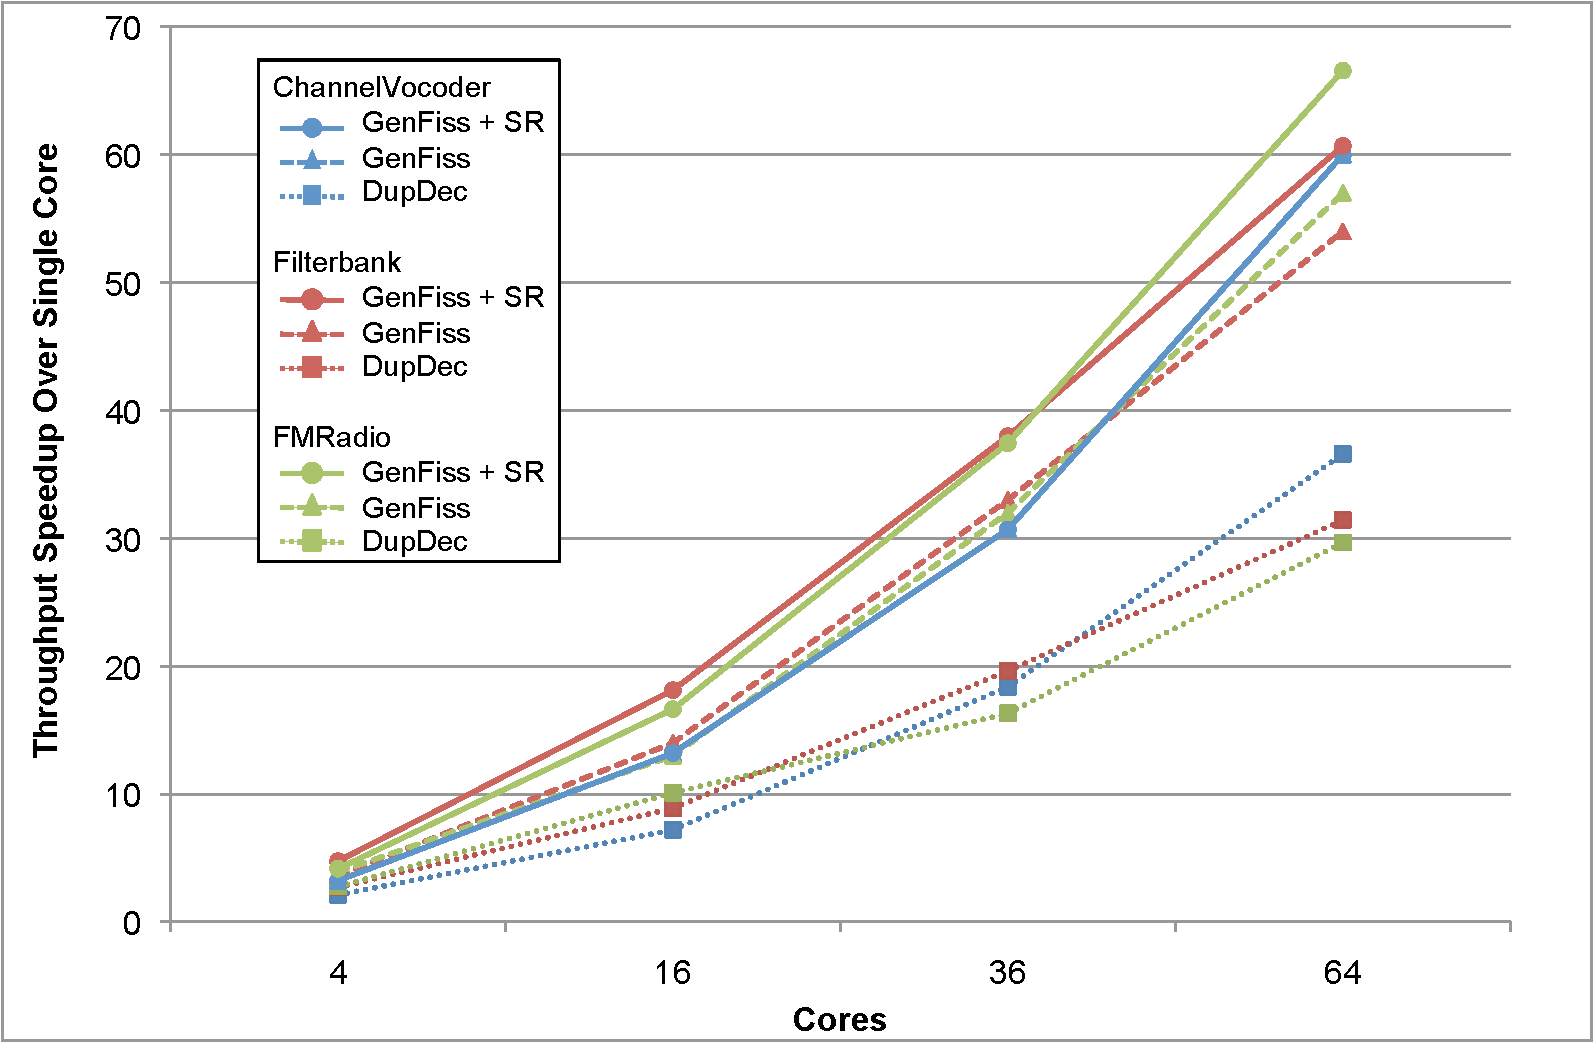
\includegraphics[width=3.3in]{figures/tilera-chart.pdf}
\caption[Comparing the fission techniques on the TILE64.]{
  Evaluation for DupDec versus general fission versus general fission with sharing reduction
  4, 16, 36, and 64 cores on the TILE64.  \label{fig:tilera-chart}}
\end{figure}

Figure~\ref{fig:tilera-chart} gives the performance results for the
Tilera TILE64 architecture.  We present results for DupDec, general
fission, and general fission with sharing reduction for 4, 16, 36, and
64 core configurations, with throughput normalized to single-core
throughput.  General fission with sharing reduction outperforms
DupDec by an average of 1.8x for the three benchmarks when targeting
64 cores. The average 64-core speedup over single core is 62.3x for the
general fission plus sharing reduction for these three benchmarks.

FMRadio experiences the most significant gain from general fission
plus sharing reduction over DupDec (67x versus 30x, respectively, for
64 cores).  FMRadio has the lowest computation to communication ratio
of the 3 benchmarks.  Furthermore, each filter of is fissed by the
number of cores targeted.  For 64 cores, each filter is fissed 64
ways.  DupDec must perform a global all-to-all communication involving
all 64 cores between each level of the graph!
 
ChannelVocoder achieves a 60x speedup for general fission over a
single core.  This is not perfectly linear because of the parallel
mapping; asymmetries exist between the extent of task parallelism and
the number of cores (see~\ref{mgordon-asplos06}).  The speedup over
DupDec (1.62x) is more modest because the width of many of the
fission applications is 3, so DupDec is duplicating input data to
groups of 3 filters.  Filterbank is similar, the width of fission is 4
for all filters when targeting 64 cores.

Sharing reduction is required to achieve scalable speedups for both
FMRadio and Filterbank.  For FMRadio, sharing reductions leads to a
17\% speedup increase for 64 cores.  This because sharing reduction
significantly reduces the number of remote write store instructions
required per output.  This affects FMRadio because of its low
computation to communication ratio.  Sharing reduction sees a 12\%
increase on Filterbank, as Filterbank has a larger computation to
communication ratio.

\begin{figure}[t]
\centering
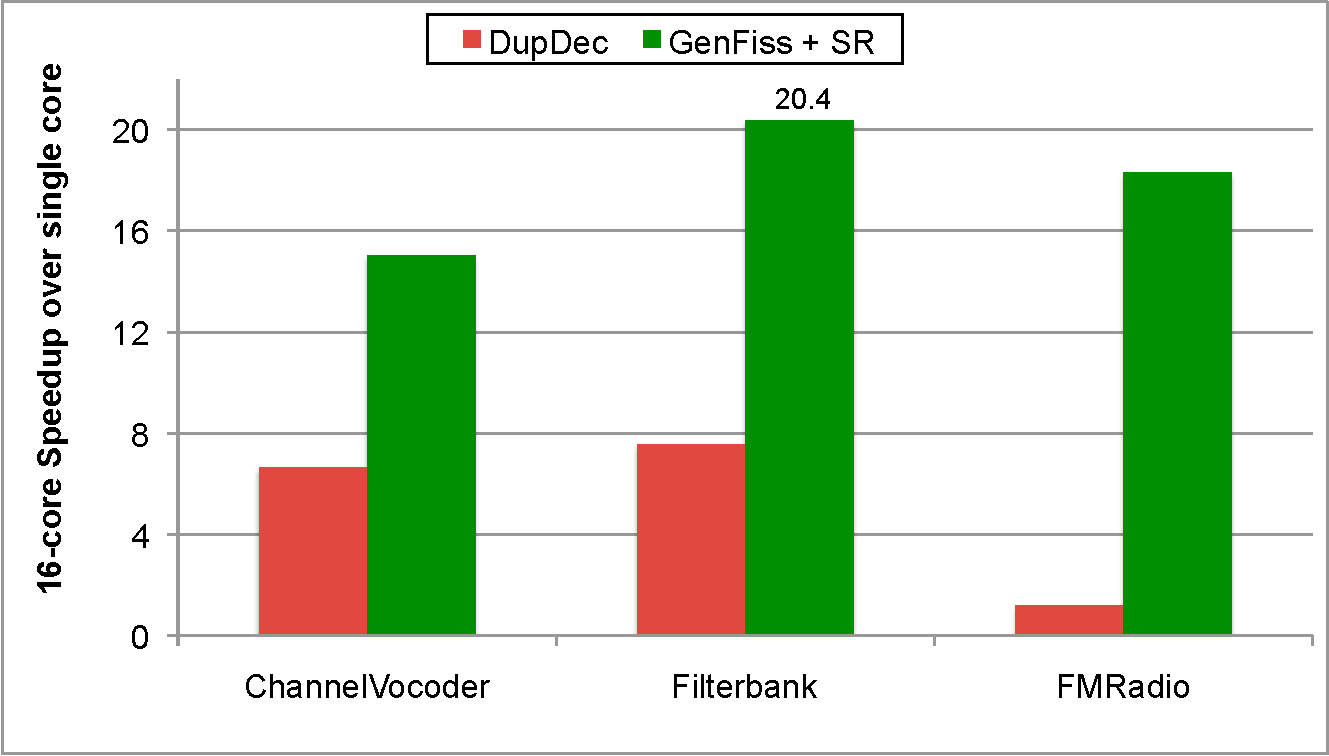
\includegraphics[width=3.3in]{figures/smp-chart.pdf}
\caption[Comparing the fission techniques on the 16-core SMP.]{
  Evaluation for DupDec versus general fission with sharing reduction
  for the 16-core SMP architecture.  \label{fig:smp-chart}}
\end{figure}

Our techniques enable scalable parallelization, with a mean speedup of
17x for our 3 benchmarks on the SMP.  Figure~\ref{fig:smp-chart} gives
the 16-core speedup comparison for DupDec versus general fission with
sharing reduction for our target SMP architecture.  The mean speedup
increase for general fission with sharing reduction over DupDec is
6.7x.  FMRadio again sees the largest speedup increase in the
comparison at 13.0x.  The reasons for this large speedup are similar
as given in the previous section.  However, the SMP communication
mechanism is not as efficient as the TILE64, thus general fission with
sharing reduction gives a greater speedup because reducing inter-core
communication has more impact.

  \section{Related Work}
\label{sec:related}

% BILL

%Signal~\cite{Signal}, 
%Lucid~\cite{Lucid77}, and
%Occam~\cite{Occam}, and Sisal \cite{sisal}.
%Parallel Haskell~\cite{ph}
In addition to StreamIt, there are a number of stream-oriented
languages drawing from domains such as functional, dataflow, CSP and
synchronous programming~\cite{survey97}.  The Brook language is
architecture-independent and focusses on data
parallelism~\cite{brook04}.  Stream kernels are required to be
stateless, though there is special support for reducing streams to a
single value.  Stream\-C/Ker\-nel\-C is lower level than Brook;
kernels written in KernelC are stiched together in StreamC and mapped
to the data-parallel Imagine processor~\cite{imagine03ieee}.  SPUR
adopts a similar decomposition between ``microcode'' stream kernels
and skeleton programs to expose data parallelism~\cite{spur05samos}.
Cg exploits pipeline parallelism and data parallelism, though the
programmer must write algorithms to exactly match the two pipeline
stages of a graphics processor~\cite{cg03}.  Compared to these
languages, StreamIt places more emphasis on exposing task and pipeline
parallelism (all the languages expose data parallelim).
%and on sliding window operations (filters that peek).  
By adopting the synchronous dataflow model of execution~\cite{lee87},
StreamIt focusses on well-structured programs that can be aggressively
optimized.  The implicit infinite loop around programs is also a key
StreamIt characteristic that enables the transformations in this
paper.  Spidle is also a recent stream language that was influenced by
StreamIt~\cite{spidle03}.
%and Lucid Synchrone~\cite{Lucid-Synchrone}.
%Synchronous languages which
%target embedded applications include Esterel~\cite{Esterel},
%Lustre~\cite{Lustre}, and Additional

Liao et al. map Brook to multicore processors by leveraging the affine
partitioning model~\cite{liao06brook}.  While affine partitioning is a
powerful model for parameterized loop-based programs, in StreamIt we
simplify the problem by fully resolving the program structure at
compile time.  This allows us to schedule a single steady state using
flexible, non-affine techniques (e.g., simulated annealing) and to
repeat the found schedule for an indefinite period at runtime.
Gummaraju and Rosenblum map stream programs to a general-purpose
hyperthreaded processor~\cite{gummaraju05micro}.  Such techniques
could be integrated with our spatial partitioning to optimize per-core
performance.  Gu et al. expose data and pipeline parallelism in a
Java-like language and use a compiler analysis to efficiently extract
coarse-grained filter boundaries~\cite{du03sc}.  Ottoni et al. also
extract decoupled threads from sequential code, using hardware-based
software pipelining to distribute the resulting threads across
cores~\cite{ottoni05decoupled}.  By embedding pipeline-parallel
filters in the programming model, we focus on the mapping step.

%%%%%%%%%%%%%%%%%%%%%%%%%%%%%%%%%%%%%%%%%%%%%%%%%%%%%%%%%%%%%%%%%%%%%

Previous work in scheduling computation graphs to parallel targets has
focused on partitioning and scheduling techniques that exploit task
and pipeline parallelism~\cite{SDFSched, SDFSched2,may87communicating,
DAGSched, pipeline-sdf}.  Application of loop-conscious
transformations to coarse-grained dataflow graphs has been
investigated.  Unrolling (or ``unfolding'' in this domain) is employed
for synchronous dataflow (SDF) graphs to reduce the initiation
interval but they do not evaluate mappings to actual
architectures~\cite{unfolding,unfolding2}. Software pipelining
techniques have been applied to SDF graphs onto various embedded and
DSP targets~\cite{bakshi99,chatha-02}, but has required programmer
knowledge of both the application and the architecture. To our
knowledge, none of these systems automatically exploit the combination
of task, data, and pipeline parallelism.  Furthermore, these systems
do not provide a robust end-to-end path for application
parallelization from a high-level, portable programming language.

%% Previous work on instruction-level software pipelining has focused
%% mostly on scheduling machine instructions in a loop via modulo
%% scheduling~\cite{rau81,lam-softpipe}.  The algorithms devised must
%% account for tight resource constraints and complex instruction
%% dependences. Our software-pipelining problem is much less constrained,
%% enabling us to employ a simple greedy heuristic.  

%% Furthermore, a traditional modulo scheduling algorithm is not needed
%% because we have an implicit loop barrier at the end of each
%% steady-state.  ILP compilers for clustered VLIW
%% architectures~\cite{Bulldog,Multiflow,lee98spacetime,qian02} must
%% partition instructions and assign them to clusters as part of the
%% instruction scheduling. Clustering is analogous to our application of
%% filter fusion in our software pipelining algorithm.

  \section{Conclusion}
\label{sec:conclusion}

In this paper, we describe the StreamIt compiler for the Raw
architecture.  The stream graph of a StreamIt program exposes the data
communication pattern to the compiler while the lack of global
synchronization frees the compiler to radically reoganize the program
for efficient execution on the underline architecture. The StreamIt
compiler demonstrates the power of this flexibility by totally
reoganizing large programs for better load balance. We were able to
map many of programs on to the Raw processor and obtain good
performance.

We introduce a collection of optimizations, vertical and horizontal
filter fusion, vertical and horizontal filter fission and filter
reordering transformations, that can be used to restructure stream
graphs.  We show that by applying these transformations we can map a
high-level stream program, written to reflect the composition of the
application, onto Raw and achieve good processor utilization and load
balance, leading to a factor of three speedup on two applications.

Unlike all previous streaming languages, the structured streams of
StreamIt makes it possible for us to approach the optimization and
parallelization problems in a very systermatic manner. It enables us
to define multiple optimizations -- targetting different constructs
and requirements -- and to compose them them in a hirearchical manner.

The ability to do global transformations across multiple filters, that
may have originated from very different parts of the application,
makes it possible for the compiler to find optimization opportunities
that may ellude even an experience programmer.  Such capabilities
enables the programmers to write protable streaming applications and
map them efficiently onto any given architecture. This has the
potential of creating a programming standard for emerging
communication exposed architectures.  The StreamIt compiler takes a
fist step towards this goal.


%  \section{Non-Hierarchical  Transformations}

\section{Non-Hierarchical Graph Transformations}

\subsection{Vertical SplitJoin Fission}

Can pull out a node from a splitjoin.

\subsection{}

\subsection{Unstructured Syncronization Removal}


\section{Non-Hierarchical Cost Functions}

\subsubsection{Layout}

\subsubsection{Communication}






  \clearpage
  \begin{figure}[t]
    \psfig{figure=algorithm4.eps,width=3.3in}
    \caption{Vertical cut algorithms.
    \protect\label{code:vert}}
  \end{figure}
  \begin{figure}[t]
    \psfig{figure=refactor2.eps,width=1.75in}
    \psfig{figure=refactor1.eps,width=1.75in}
    \caption{Vertical cut example.
    \protect\label{ex:vert}}
  \end{figure}
  
  \clearpage
  \begin{figure}[t]
    \psfig{figure=algorithm5.eps,width=3.5in}
    \caption{Horizontal cut algorithms.
    \protect\label{code:horiz}}
  \end{figure}
  \begin{figure}[t]
    \psfig{figure=matchsync2.eps,width=1.75in}
    \psfig{figure=matchsync1.eps,width=1.75in}
    \caption{Horizontal cut example.
      \protect\label{ex:horiz}}
  \end{figure}
  
  \clearpage
  \begin{figure}[t]
    \psfig{figure=algorithm6.eps,width=3.5in}
    \caption{Aggressive synchronization removal.
    \protect\label{code:syc}}
  \end{figure}
  \begin{figure}[t]
    \psfig{figure=sync2.eps,width=1.75in}
    \psfig{figure=sync1.eps,width=1.75in}
    \caption{Example of synchronization removal.
    \protect\label{ex:sync}}
  \end{figure}
  
  
  \clearpage
  \begin{figure*}[t]
    \begin{tabular}{ll}
    \psfig{figure=algorithm.eps,width=3.5in}
    &
    \psfig{figure=algorithm2.eps,width=3.5in}
    \end{tabular}
    \caption{Search phase of the partitioning algorithm.  The traceback phase appears in the appendix.
      \protect\label{code:partition}}
  \end{figure*}

  \section*{Appendix}
  \begin{figure}[t]
    \psfig{figure=algorithm3.eps,width=3.5in}
  \end{figure}
  
  % Bibliography -- whee!
  \begin{small}
    \bibliographystyle{abbrv}
    \bibliography{references}
  \end{small}
  
\end{document}